\section{Results}
\label{sec:results}

All 320 cells of the US sweep passed the placement check of
Section~\ref{sec:validity}: every virtual machine executed in the region its
planner selected, and every cloudlet completed within the measurement window.
Figures are reported on the attributed basis of Eq.~\eqref{eq:attr} unless
stated otherwise, with the dynamic basis of Eq.~\eqref{eq:dyn} given alongside
where the two diverge. Spreads are standard deviations across the five workload
samples.

\subsection{Capacity utilisation determines the value of deadline flexibility}
\label{sec:res-capacity}

Table~\ref{tab:capmargin} reports emissions for the joint space-and-time policy
across the capacity and deadline-margin grid. Reading down a column gives the
effect of capacity at fixed flexibility; reading across a row gives the effect
of flexibility at fixed capacity.

\begin{table}[t]
\centering
\caption{Attributed emissions (kgCO\textsubscript{2}eq) for space+time
scheduling, mean across five workload samples with standard deviation in
parentheses. Utilisation is total demand divided by total available slot-hours.}
\label{tab:capmargin}
\begin{tabular}{llrrrr}
\toprule
& & \multicolumn{4}{c}{Deadline margin (h)} \\
\cmidrule(l){3-6}
Capacity & Utilisation & 6 & 12 & 24 & 48 \\
\midrule
 56 & 82\,\% & 2065 (138) & 2067 (131) & 2059 (131) & 2047 (134) \\
 84 & 55\,\% & 1821 (117) & 1787 (128) & 1755 (128) & 1718 (127) \\
140 & 33\,\% & 1421 (102) & 1390 (107) & 1350 (108) & 1321 (110) \\
350 & 13\,\% &  683\ (88) &  555 (119) &  484\ (95) &  463\ (71) \\
\bottomrule
\end{tabular}
\end{table}

The two effects differ by more than an order of magnitude. Increasing capacity
from 56 to 350 slots reduces emissions by 77.4\,\% $\pm$ 2.3 at the widest
deadline margin, and the reduction is between 66.1\,\% and 77.4\,\% at every
margin considered. Increasing the deadline margin from 6\,h to 48\,h reduces
emissions by 32.1\,\% $\pm$ 6.1 at the lowest utilisation but by only
0.9\,\% $\pm$ 0.6 at the highest.

The value of deadline flexibility is therefore not a property of the workload
or of the scheduler alone; it is conditional on how heavily the system is
loaded. Table~\ref{tab:marginbyutil} states this dependence directly.

\begin{figure}[t]
\centering
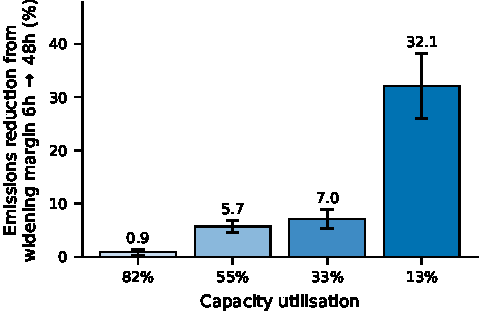
\includegraphics{figures/fig_margin_by_utilisation.pdf}
\caption{The value of deadline flexibility is conditional on load. Bars show the
reduction in attributed emissions obtained by widening the deadline margin from
6\,h to 48\,h under space+time scheduling; error bars are one standard deviation
across five workload samples.}
\label{fig:margin}
\end{figure}

\begin{table}[t]
\centering
\caption{Reduction in attributed emissions obtained by widening the deadline
margin from 6\,h to 48\,h, by capacity utilisation. Mean and standard deviation
across five workload samples.}
\label{tab:marginbyutil}
\begin{tabular}{lr}
\toprule
Capacity utilisation & Reduction from 6\,h to 48\,h margin \\
\midrule
82\,\% & \phantom{0}0.9\,\% $\pm$ 0.6 \\
55\,\% & \phantom{0}5.7\,\% $\pm$ 1.2 \\
33\,\% & \phantom{0}7.0\,\% $\pm$ 1.8 \\
13\,\% & 32.1\,\% $\pm$ 6.1 \\
\bottomrule
\end{tabular}
\end{table}

At 82\,\% utilisation the effect of deadline margin is 1.5 standard deviations
from zero and is not distinguishable from no effect at any conventional
threshold. The interpretation is mechanical rather than statistical: deferring a
request is only useful if a cleaner slot is free when the request is ready to
move, and under heavy load the cleaner slots are already occupied. Flexibility
that cannot be exercised has no value.

The saturated row of Table~\ref{tab:capmargin} carries a second qualification.
At 56 slots, between 152 and 408 of the 1\,000 requests miss their deadlines
depending on policy and margin, whereas at 84 slots and above no request does.
Emissions comparisons in the saturated regime therefore compare schedules that
are all failing, and we report that row as a boundary condition rather than as
an operating point.

\subsection{Time shifting is dominated by the choice of origin region}
\label{sec:res-home}

WaitAwhile~\cite{wiesner2021letswait} defers requests within a fixed origin region. Its reported
performance therefore depends on which region that is. We instantiate the
policy once per region of the set and examine what predicts the outcome.

Across all four capacity and margin combinations, the correlation between the
mean carbon intensity of the origin region and the emissions the policy achieves
is between $+0.941$ and $+0.998$, with a standard deviation across workload
samples of at most $0.017$. The correlation between the origin region's diurnal
amplitude and the same emissions is between $-0.066$ and $+0.085$, in every case
within one standard deviation of zero. Table~\ref{tab:homecorr} reports both.

\begin{table}[t]
\centering
\caption{What predicts WaitAwhile's emissions. Pearson correlation between the
policy's attributed emissions and two properties of its origin region, across
the seven regions of the US set. Mean and standard deviation over five workload
samples.}
\label{tab:homecorr}
\begin{tabular}{llrr}
\toprule
Capacity & Margin (h) & Origin mean CI & Origin diurnal amplitude \\
\midrule
 84 &  6 & $+0.953 \pm 0.017$ & $-0.066 \pm 0.067$ \\
 84 & 48 & $+0.941 \pm 0.016$ & $-0.007 \pm 0.076$ \\
350 &  6 & $+0.989 \pm 0.006$ & $+0.056 \pm 0.026$ \\
350 & 48 & $+0.998 \pm 0.002$ & $+0.085 \pm 0.020$ \\
\bottomrule
\end{tabular}
\end{table}

The policy's outcome is thus determined by how clean its origin grid is and not
by how much daily variation that grid offers, even though daily variation is
the only quantity the policy acts upon. The US set contains a region, CISO,
whose diurnal amplitude of 52.7\,\% is more than six times that of the flattest
region in the set; instantiating WaitAwhile there yields no advantage over
instantiating it in a region of comparable mean intensity and a quarter of the
amplitude.

The practical consequence is the spread in Table~\ref{tab:homespread}. At the
lowest utilisation, the best origin region yields 467\,kgCO\textsubscript{2}eq
and the worst 1705, a factor of 3.6. Space shifting, which is free to choose its
region per request, yields 701. The best available origin outperforms space
shifting; the median origin is worse than it by a factor of two.

\begin{figure*}[t]
\centering
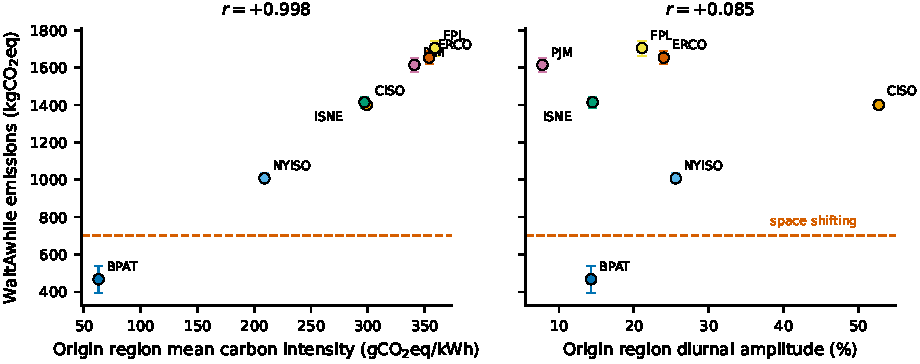
\includegraphics{figures/fig_home_region.pdf}
\caption{WaitAwhile emissions against two properties of the origin region, at
350 slots and a 48\,h margin. Each point is one of the seven candidate origins,
averaged over five workload samples; error bars are one standard deviation. The
dashed line marks space shifting in the same cell. The policy's outcome tracks
the origin's mean carbon intensity (left) and not its diurnal amplitude (right),
although the latter is the only quantity the policy acts upon.}
\label{fig:home}
\end{figure*}

\begin{table}[t]
\centering
\caption{WaitAwhile attributed emissions (kgCO\textsubscript{2}eq) across the
seven possible origin regions, with space shifting for comparison. Values are
means over five workload samples.}
\label{tab:homespread}
\begin{tabular}{llrrrr}
\toprule
Capacity & Margin (h) & Best origin & Median origin & Worst origin & Space \\
\midrule
 84 &  6 & 1841 & 1974 & 2039 & 1857 \\
 84 & 48 & 1781 & 1905 & 1984 & 1857 \\
350 &  6 &  683 & 1432 & 1698 &  701 \\
350 & 48 &  467 & 1415 & 1705 &  701 \\
\bottomrule
\end{tabular}
\end{table}

A single reported figure for a time-shifting policy is therefore a draw from a
distribution whose width exceeds the difference between the policies being
compared, and the draw is determined by a parameter that evaluations do not
customarily state. Prior work on the limits of temporal shifting
\cite{sukprasert2024limitations} does not isolate this parameter. In both region sets examined here, the conventional choice of
the first region in the candidate list happens to select the cleanest grid
available, which assigns the policy the most favourable draw.

\subsection{Reported savings scale with the composition of the region set}
\label{sec:res-regionset}

The same workload and the same scheduler were run over two region sets at
matched capacity utilisation. Table~\ref{tab:regionset} reports the reduction
that space shifting achieves relative to the carbon-agnostic baseline in each.

\begin{figure}[t]
\centering
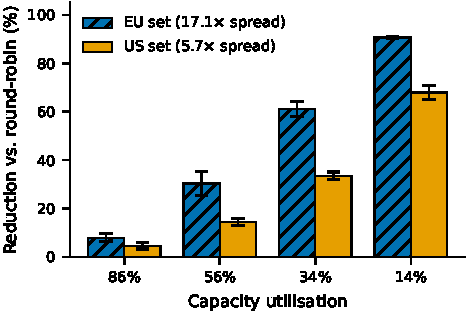
\includegraphics{figures/fig_region_set.pdf}
\caption{Reported savings scale with the composition of the candidate region
set. Identical workload, scheduler and hardware; the sets differ only in the
ratio between their cleanest region and the next cleanest. Error bars are one
standard deviation across workload samples.}
\label{fig:regionset}
\end{figure}

\begin{table}[t]
\centering
\caption{Reduction in attributed emissions from space shifting relative to
round-robin placement, at matched capacity utilisation, for two region sets.
Mean and standard deviation across workload samples (five for US, three for EU).}
\label{tab:regionset}
\begin{tabular}{lrr}
\toprule
Capacity utilisation & EU set & US set \\
\midrule
86\,\% & \phantom{0}7.8\,\% $\pm$ 1.6 & \phantom{0}4.6\,\% $\pm$ 1.4 \\
56\,\% & 30.3\,\% $\pm$ 4.9 & 14.3\,\% $\pm$ 1.5 \\
34\,\% & 61.1\,\% $\pm$ 3.2 & 33.4\,\% $\pm$ 1.6 \\
14\,\% & 90.7\,\% $\pm$ 0.4 & 67.9\,\% $\pm$ 3.0 \\
\bottomrule
\end{tabular}
\end{table}

The EU set reports roughly twice the reduction of the US set at every operating
point, and the difference exceeds the combined standard deviations in all four
rows. Nothing about the scheduler, the workload or the amount of hardware
differs between the two columns. The difference is the composition of the
candidate set: the EU set contains a region 4.7 times cleaner than its nearest
rival, so that a single destination is optimal for almost every request, whereas
in the US set the corresponding ratio is 3.3 and the placement decision remains
contested.

Regional concentration confirms the mechanism, and
Figure~\ref{fig:concentration} shows it directly. Across all valid cells of both
sets, the correlation between the share of the workload placed in the busiest
region and attributed emissions is $-0.930$ for the US set and $-0.963$ for the
EU set. In the EU set at the lowest utilisation, space shifting places 98\,\% of
the workload in a single region; in the US set it places 96\,\%. The reductions
these policies report are, to a first approximation, a measure of how much of
the workload the capacity constraint permits them to move into the cleanest
available grid.

\begin{figure}[t]
\centering
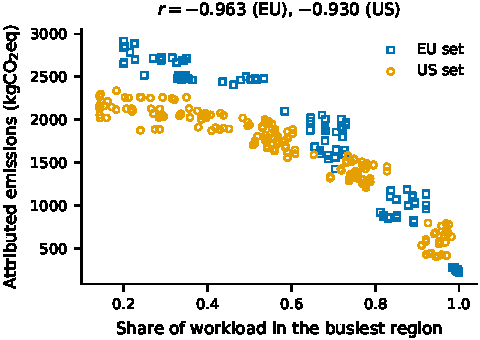
\includegraphics{figures/fig_concentration.pdf}
\caption{The mechanism common to all three findings. Each point is one
experimental cell. Emissions fall as a larger share of the workload is placed in
the busiest region, and the relationship holds across both region sets and every
capacity, deadline margin and policy examined.}
\label{fig:concentration}
\end{figure}

\subsection{Robustness}
\label{sec:res-robustness}

\paragraph{Season.} Repeating the sweep on a 720\,h window beginning in July
rather than January changes the correlation between origin carbon intensity and
WaitAwhile's emissions from the range $[+0.941, +0.998]$ to $[+0.760, +0.892]$,
and the correlation with diurnal amplitude from approximately zero to the range
$[-0.518, -0.285]$. Diurnal structure therefore acquires a secondary influence
in summer, when solar generation widens the daily cycle in several regions,
without displacing origin cleanliness as the dominant term. The ordering of
policies is unchanged.

\paragraph{Workload class.} Restricting the workload to the class the provider
labels delay-insensitive preserves the result, with the correlation between
origin carbon intensity and emissions at $+0.822$, $+0.920$ and $+0.936$ in
three of four cells. The exception is the combination of tight capacity and wide
margin, where the correlation with origin intensity falls to $+0.403$ and that
with diurnal amplitude rises to $+0.776$: when capacity constrains relocation
and the deadline permits deferral, temporal structure is the only remaining
lever and briefly becomes the dominant one.

This class also differs from the general mixture in a way that bears on the
premise of deadline-based scheduling. Its mean virtual machine lifetime is
340.7\,h against 34\,h for the unrestricted sample, an order of magnitude
longer. A 48\,h margin therefore represents 141\,\% of the mean lifetime in the
general mixture but only 14\,\% in the class explicitly designated as tolerant
of delay. The population with the most permission to wait has the least relative
room in which to do so.

\paragraph{Power model.} Repeating the entire sweep under the linear 120/480\,W
model in place of the measured curve raises absolute emissions by approximately
40\,\% but leaves every reported proportion within its sampling spread: the
capacity effect moves from 77.4\,\% $\pm$ 2.3 to 75.9\,\% $\pm$ 2.2, the margin
effect at 82\,\% utilisation from 0.9\,\% $\pm$ 0.6 to 1.0\,\% $\pm$ 0.5, the
correlation with origin intensity from $[+0.941, +0.998]$ to
$[+0.943, +0.998]$, and the EU-to-US ratio at the lowest utilisation from
90.7/67.9 to 90.1/67.1. The conclusions of
Sections~\ref{sec:res-capacity}--\ref{sec:res-regionset} are therefore not
artefacts of the power model adopted.

The absolute values are not invariant, and the direction of the change is worth
recording. Under the measured curve, round-robin placement rises by 44\,\%
while the carbon-aware policies rise by 26\,\% or less, so the reduction
attributed to space shifting increases rather than decreases. The attributed
basis charges the full draw of every host carrying load, and the measured
machine idles at 55\,\% of peak rather than 25\,\%; raising the fixed cost of
activating a host penalises the policy that activates the most. Round-robin
placement leaves 72 hosts active at the lowest utilisation against 47 for space
shifting and 38 for space+time. Part of what the attributed basis records as a
carbon-aware saving is therefore a consolidation saving. The dynamic basis,
which excludes idle draw entirely, separates the two: on that basis the same
comparison yields reductions of 64\,\% and 71\,\% respectively, confirming that
regional placement rather than consolidation accounts for the larger share.
